\subsection{Testowanie wielomianów rzadkich}

\subsubsection{Wielomiany stopnia parzystego}

Kolejnym przypadkiem jest zbadanie rzadkich wielomianów, nieposiadających pierwiastków całkowitych. By zapewnić ten element, najłatwiejszym sposobem jest konstrukcja wielomianu postaci $ax^{2k}+b$, gdzie $a \in R_+, b \in R, k \in Z_+$. Dzięki temu, mamy pewność, że wielomian nie posiada pierwiastków całkowitych, a~dodatkowo ma najmniejszą możliwą liczbę niezerowych współczynników.

Teoretycznie, wielomiany rzadkie powinny się charakteryzować największą dysproporcją w~wydajności pomiędzy typami PolynomialMap i~PolynomialVector, na korzyść tego pierwszego. Jest to spowodowane faktem, że to właśnie w~tym przypadku, odsetek zerowych współczynników jest największy. Czynnik ten powinien bardzo negatywnie wpływać na czas znajdowania pierwiastków, a~w tym przypadku na stwierdzenie, o~ich braku. Zapoznajmy się z~wynikami testów, by zweryfikować postawioną powyżej tezę.

\begin{table}[H]
	\begin{tabular}{ |p{3.5cm}|p{3cm}|p{3cm}|p{3.5cm}|} 
		\hline
		Testowany wielomian & Czas dla PolynomialMap [s] & Czas dla PolynomialVector [s] & Współczynnik czasów \\
		\hline
		$W(x) = x^{100} + 1$ & 0.003 & 0.045 & 15 \\
		$W(x) = x^{200} + 1$ & 0.004 & 0.159 & 39.75 \\
		$W(x) = x^{400} + 1$ & 0.005 & 0.647 & 129.4 \\
		$W(x) = x^{800} + 1$ & 0.017 & 2.790 & 164.12 \\
		$W(x) = x^{1600} + 1$ & 0.025 & 13.035 & 521.4 \\
		$W(x) = x^{3200} + 1$ & 0.058 & 67.311 & 1160.53 \\
		\hline
	\end{tabular}
	\caption{Porównanie czasów znajdowania pierwiastków dla rzadkich wielomianów parzystego stopnia. Źródło: opracowanie własne.}
\end{table}

Jak widać na podstawie uzyskanych czasów dla obu wielomianów dysproporcja pomiędzy ich wydajnością dla wielomianów rzadkich jest ogromna. Można zauważyć, że wraz ze wzrostem wielomianów staje się ona coraz większa. Dodatkowo, widać, że w~przypadku PolynomialVector uzyskane czasy rosną około pięciokrotnie, przy dwukrotnym wzroście stopnia wielomianu, co oznacza przekraczającą nawet kwadratową zależność.

Poniżej przedstawiam wykresy dla obu typów wielomianów. Zdecydowałem się na rozdzielenie ich na dwa osobne wykresy ze względu na wspomnianą wcześniej ogromną dysproporcję. W~przeciwnym razie na wykresie o~liniowej skali wartości czasów dla PolynomialMap byłyby tak małe, że pokrywałyby się z~osią poziomą.

\begin{figure}[H]
	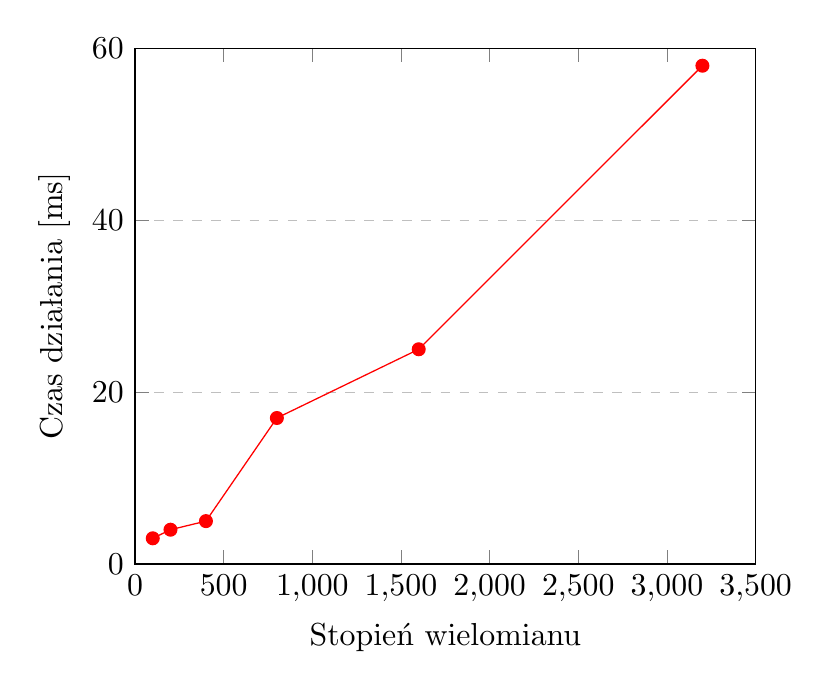
\begin{tikzpicture}[scale=1.15]
	\begin{axis}[
	xlabel={Stopień wielomianu},
	ylabel={Czas działania [ms]},
	xmin=0,xmax=3500,
	ymin=0,ymax=60,
	ymajorgrids=true,grid style=dashed
	]
	
	\addplot[color=red,mark=*]
	coordinates {
		(100, 3)
		(200, 4)
		(400, 5)
		(800, 17)
		(1600, 25)
		(3200, 58)
	};
	\end{axis}
	\end{tikzpicture}
	\caption{Czasy znajdowania pierwiastków przez PolynomialMap dla rzadkich wielomianów parzystego stopnia. Źródło: opracowanie własne.}
\end{figure}

Warto zauważyć, że wszystkie czasy przedstawione na powyższym wykresie zostały wyrażone w~milisekundach. Dodatkowo na uwagę zasługuje fakt, że również czas działania dla wielomianów bardzo wysokich stopni jest bardzo mały. Wartości te rosną w~tempie nieco wyższym niż liniowe. Oznacza to bardzo dobrą skalowalność działania algorytmu dla struktury PolynomialMap.  

\begin{figure}[H]
	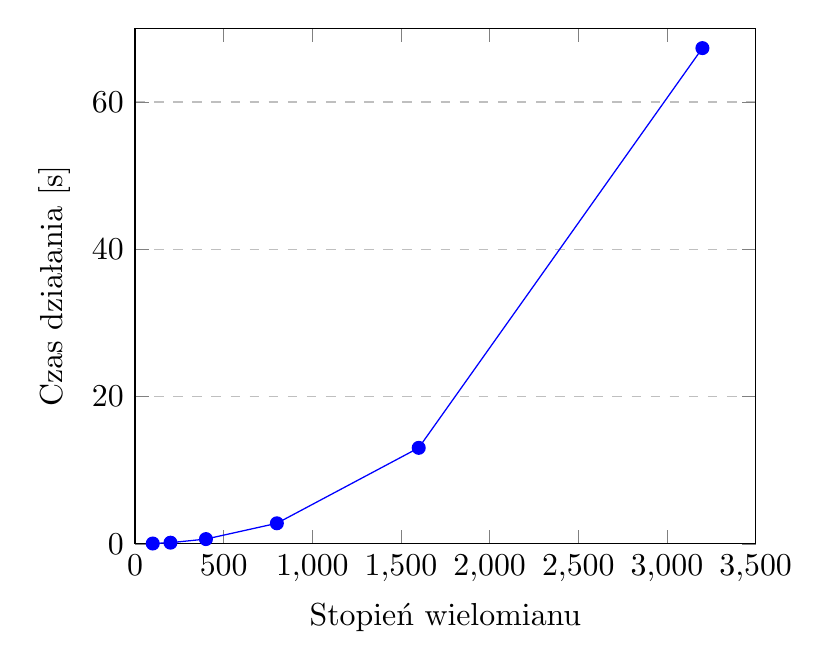
\begin{tikzpicture}[scale=1.15]
	\begin{axis}[
	xlabel={Stopień wielomianu},
	ylabel={Czas działania [s]},
	xmin=0,xmax=3500,
	ymin=0,ymax=70,
	ymajorgrids=true,grid style=dashed
	]
	\addplot[color=blue,mark=*]
	coordinates {
		(100, 0.045)
		(200, 0.159)
		(400, 0.647)
		(800, 2.79)
		(1600, 13.035)
		(3200, 67.311)	
	};
	\end{axis}
	\end{tikzpicture}
	\caption{Czasy znajdowania pierwiastków przez PolynomialVector dla rzadkich wielomianów parzystego stopnia. Źródło: opracowanie własne.}
\end{figure}

\subsubsection{Wielomiany stopnia nieparzystego}

Teraz rozpatrzmy sytuację, w~której ponownie mamy do czynienia z~wielomianem rzadkim, o~którym wiemy, że posiada przynajmniej jeden pierwiastkek rzeczywisty. By to zapewnić, wystarczy skonstruować wielomian w~postaci $ax^{2k+1}+b$, gdzie $a \in R\setminus\{0\}, b \in R, k \in Z_+$. Jak wiemy na podstawie przedstawionego w~drugim rozdziale twierdzenia, każdy wielomian stopnia nieparzystego posiada przynajmniej jeden pierwiastek rzeczywisty. 

Wydaje się, że podobnie jak w~przypadku wielomianów nieposiadających pierwiastków, również w~tym, czas znajdowania pierwiastków dla typu PolynomialMap powinien być znacznie krótszy niż dla PolynomialVector. Aby to potwierdzić, postarajmy się zbudować ciąg Sturma dla wielomianu $x^{101}+1$. Zacznijmy od obliczenia pochodnej. $(x^{101}+1)'=101x^{100}$. Obliczona wartość jest drugim elementem ciągu Sturma. Obliczmy resztę z~dzielenia dwóch pierwszych wielomianów tego ciągu.

\begin{equation*}
\begin{split}
&\frac{1}{101}x \\
\hline
&(x^{101}+1) : (101x^{100}) \\
&-x^{101} \\
\hline
&1
\end{split}
\end{equation*}

Trzecim i~jednocześnie ostatnim wyrazem ciągu Sturma jest więc $-1$, czyli wartość przeciwna do otrzymanej reszty. Dysponujemy zatem trzywyrazowym ciągiem Sturma o~elementach ${x^{101}+1, 101x^{100}, -1}$. Obliczmy teraz liczbę zmian znaków dla bardzo dużych wartości bezwzględnych, dążących odpowiednio do $-\infty$ i~$+\infty$. W~prawym krańcu przedziału będą to wartości $+,+,-,$ zaś w~lewym $-,+,-.$ Otrzymaliśmy odpowiednio jedną i dwie zmiany znaku. Oznacza to, że liczba pierwiastków rzeczywistych jest równa różnicy tych zmian w~lewym i~prawym krańcu, czyli w~tym przypadku wynosi $1$. Jak widać, dwa z~trzech elementów ciągu Sturma to rzadkie wielomiany wysokich stopni. Na takiej podstawie, wydaje się, że powyższa teza została potwierdzona. Jednocześnie jednak, warto zauważyć, że dla tego rodzaju wielomianów liczba koniecznych operacji jest niewielka, z~uwagi na znikomą liczbę elementów ciągu Sturma. Wydaje się zatem, że to właśnie ich liczba bezpośrednio wpływa na czas znajdowania pierwiastków, a~ich charakterystyka, czyli liczba niezerowych współczynników ma największe znaczenie dla wydajności obu typów wielomianów.

\begin{table}[H]
	\begin{tabular}{ |p{3.5cm}|p{3cm}|p{3cm}|p{3.5cm}|} 
		\hline
		Testowany wielomian & Czas dla PolynomialMap [s] & Czas dla PolynomialVector [s] & Współczynnik czasów \\
		\hline
		$W(x) = x^{101} + 1$ & 0.049 & 2.278 & 46.49 \\
		$W(x) = x^{201} + 1$ & 0.102 & 9.438 & 92.53 \\
		$W(x) = x^{401} + 1$ & 0.221 & 40.432 & 182.95 \\
		$W(x) = x^{801} + 1$ & 0.525 & 184.608 & 351.63 \\
		$W(x) = x^{1601} + 1$ & 1.374 & 912.716 & 664.28 \\
		$W(x) = x^{3201} + 1$ & 4.153 & 5125.106 & 1234.07 \\
		\hline
	\end{tabular}
	\caption{Porównanie czasów znajdowania pierwiastków dla rzadkich wielomianów nieparzystego stopnia. Źródło: opracowanie własne.}
\end{table}

Jak widać również w~tym przypadku zauważalna jest niesamowita różnicą między wydajnością działania obu struktur. Dodatkowo również ten test potwierdza, że nieparzysty stopień wielomianu powoduje wielokrotne wydłużenie czasu trwania algorytmu.

Poniżej przedstawiam wykresy z~czasami działania obu struktur.

\begin{figure}[H]
	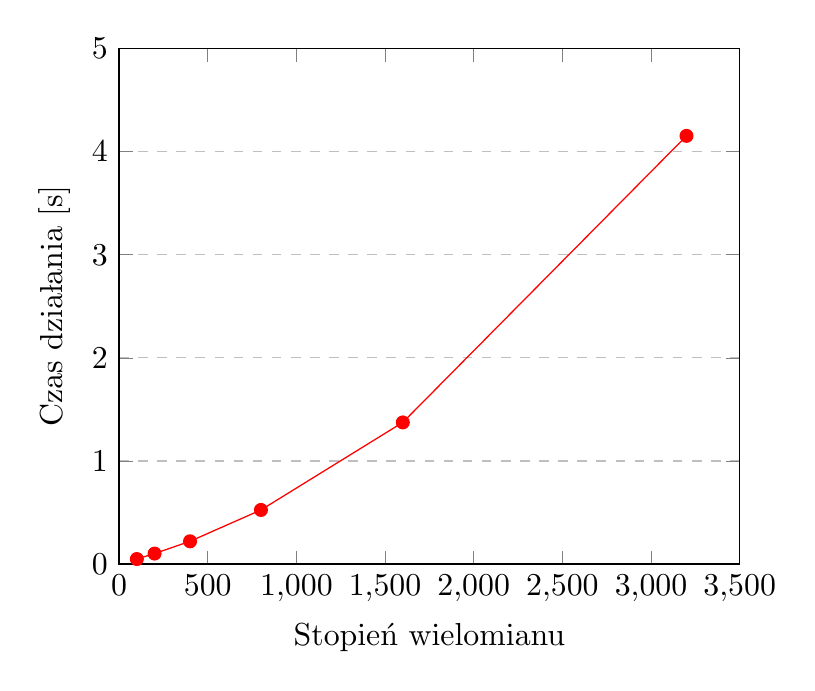
\begin{tikzpicture}[scale=1.15]
	\begin{axis}[
	xlabel={Stopień wielomianu},
	ylabel={Czas działania [s]},
	xmin=0,xmax=3500,
	ymin=0,ymax=5,
	ymajorgrids=true,grid style=dashed
	]
	
	\addplot[color=red,mark=*]
	coordinates {
		(100, 0.049)
		(200, 0.102)
		(400, 0.221)
		(800, 0.525)
		(1600, 1.374)
		(3200, 4.153)
	};
	\end{axis}
	\end{tikzpicture}
	\caption{Czasy znajdowania pierwiastków przez PolynomialMap dla rzadkich wielomianów nieparzystego stopnia. Źródło: opracowanie własne.}
\end{figure}

\begin{figure}[H]
	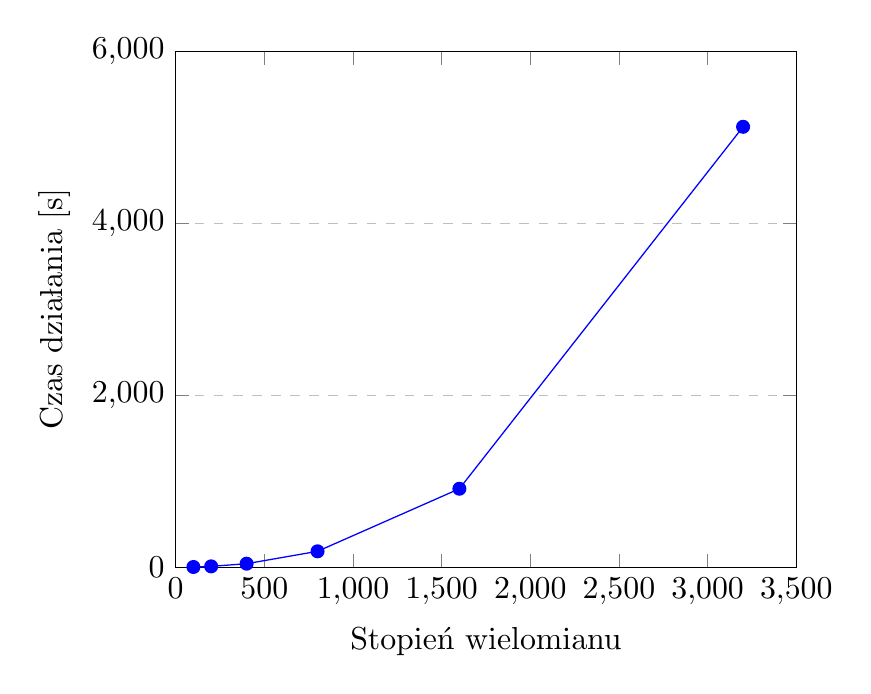
\begin{tikzpicture}[scale=1.15]
	\begin{axis}[
	xlabel={Stopień wielomianu},
	ylabel={Czas działania [s]},
	xmin=0,xmax=3500,
	ymin=0,ymax=6000,
	ymajorgrids=true,grid style=dashed
	]
	
	\addplot[color=blue,mark=*]
	coordinates {
		(100, 2.278)
		(200, 9.438)
		(400, 40.432)
		(800, 184.608)
		(1600, 912.716)
		(3200, 5125.106)	
	};
	\end{axis}
	\end{tikzpicture}
	\caption{Czasy znajdowania pierwiastków przez PolynomialVector dla rzadkich wielomianów nieparzystego stopnia. Źródło: opracowanie własne.}
\end{figure}

Można zauważyć, że czasy działania w~przypadku obu struktur są zdecydowanie krótsze niż dla wielomianów gęstych. Mniejszą różnicę obserwujemy dla typu PolynomialVector. Jej istnienie jest spowodowane faktem, że w~obu przypadkach musimy przejrzeć kolejne współczynniki, ale większość reakcji wymaga dodatkowego działania wyłącznie wtedy, gdy są one niezerowe.

Zdecydowanie większa dysproporcja jest w~przypadku klasy PolynomialMap. Wynika ona z~konieczności dodatkowych obliczeń dla kolejnych współczynników, a~oprócz tego wymusza przetrzymywanie informacji o~ich wartości.
